\section[PROJETO DE UM DISPOSITIVO (ENTREGA 4)]{PROJETO DE UM DISPOSITIVO: GABARITO DE COLAGEM DO ÍMÃ (ENTREGA~4)}\label{sec:projeto_dispositivo}

O planejamento do processo aponta os dispositivos e as ferramentas especiais de que as operações precisam, e o projeto desses recursos faz parte do projeto detalhado \cite{rozenfeld2006gestao}. Entre os recursos específicos do Tag\&Go listados no plano macro (Tabela~\ref{tab:plano_recursos}), a equipe escolheu projetar o gabarito de colagem do ímã no braço, usado no Posto~0. Ele atende ao braço, um item crítico, e é o único recurso que fixa uma cota funcional do produto sem ter equivalente no mercado: a altura de 11,80~mm entre a face polar do ímã e a face do braço, uma das três parcelas da folga (Tabela~\ref{tab:des_cadeia}).

\subsection{Solução}
\label{subsec:disp_solucao}

O gabarito inverte a montagem (Figura~\ref{fig:fd01}). No produto, o ímã fica sobre o braço. No gabarito, ele entra primeiro, com a face polar para baixo, num ninho de 11,80~mm de profundidade, e o braço é colocado por cima, com o alojamento voltado para o ímã. O fundo do ninho e a face da placa viram as duas referências da cota. Como o ímã tem 12~mm, ele sobressai 0,20~mm e entra no alojamento de 0,50~mm do braço, e os 0,30~mm restantes ficam para o adesivo. Se o ímã vier um pouco mais alto ou mais baixo, a linha de adesivo absorve a diferença e a cota não muda.

\begin{landscape}
\begin{figure}[p]
    \centering
    \caption{Desenho esquemático do gabarito de colagem do ímã no braço (FD-01)}
    \label{fig:fd01}
    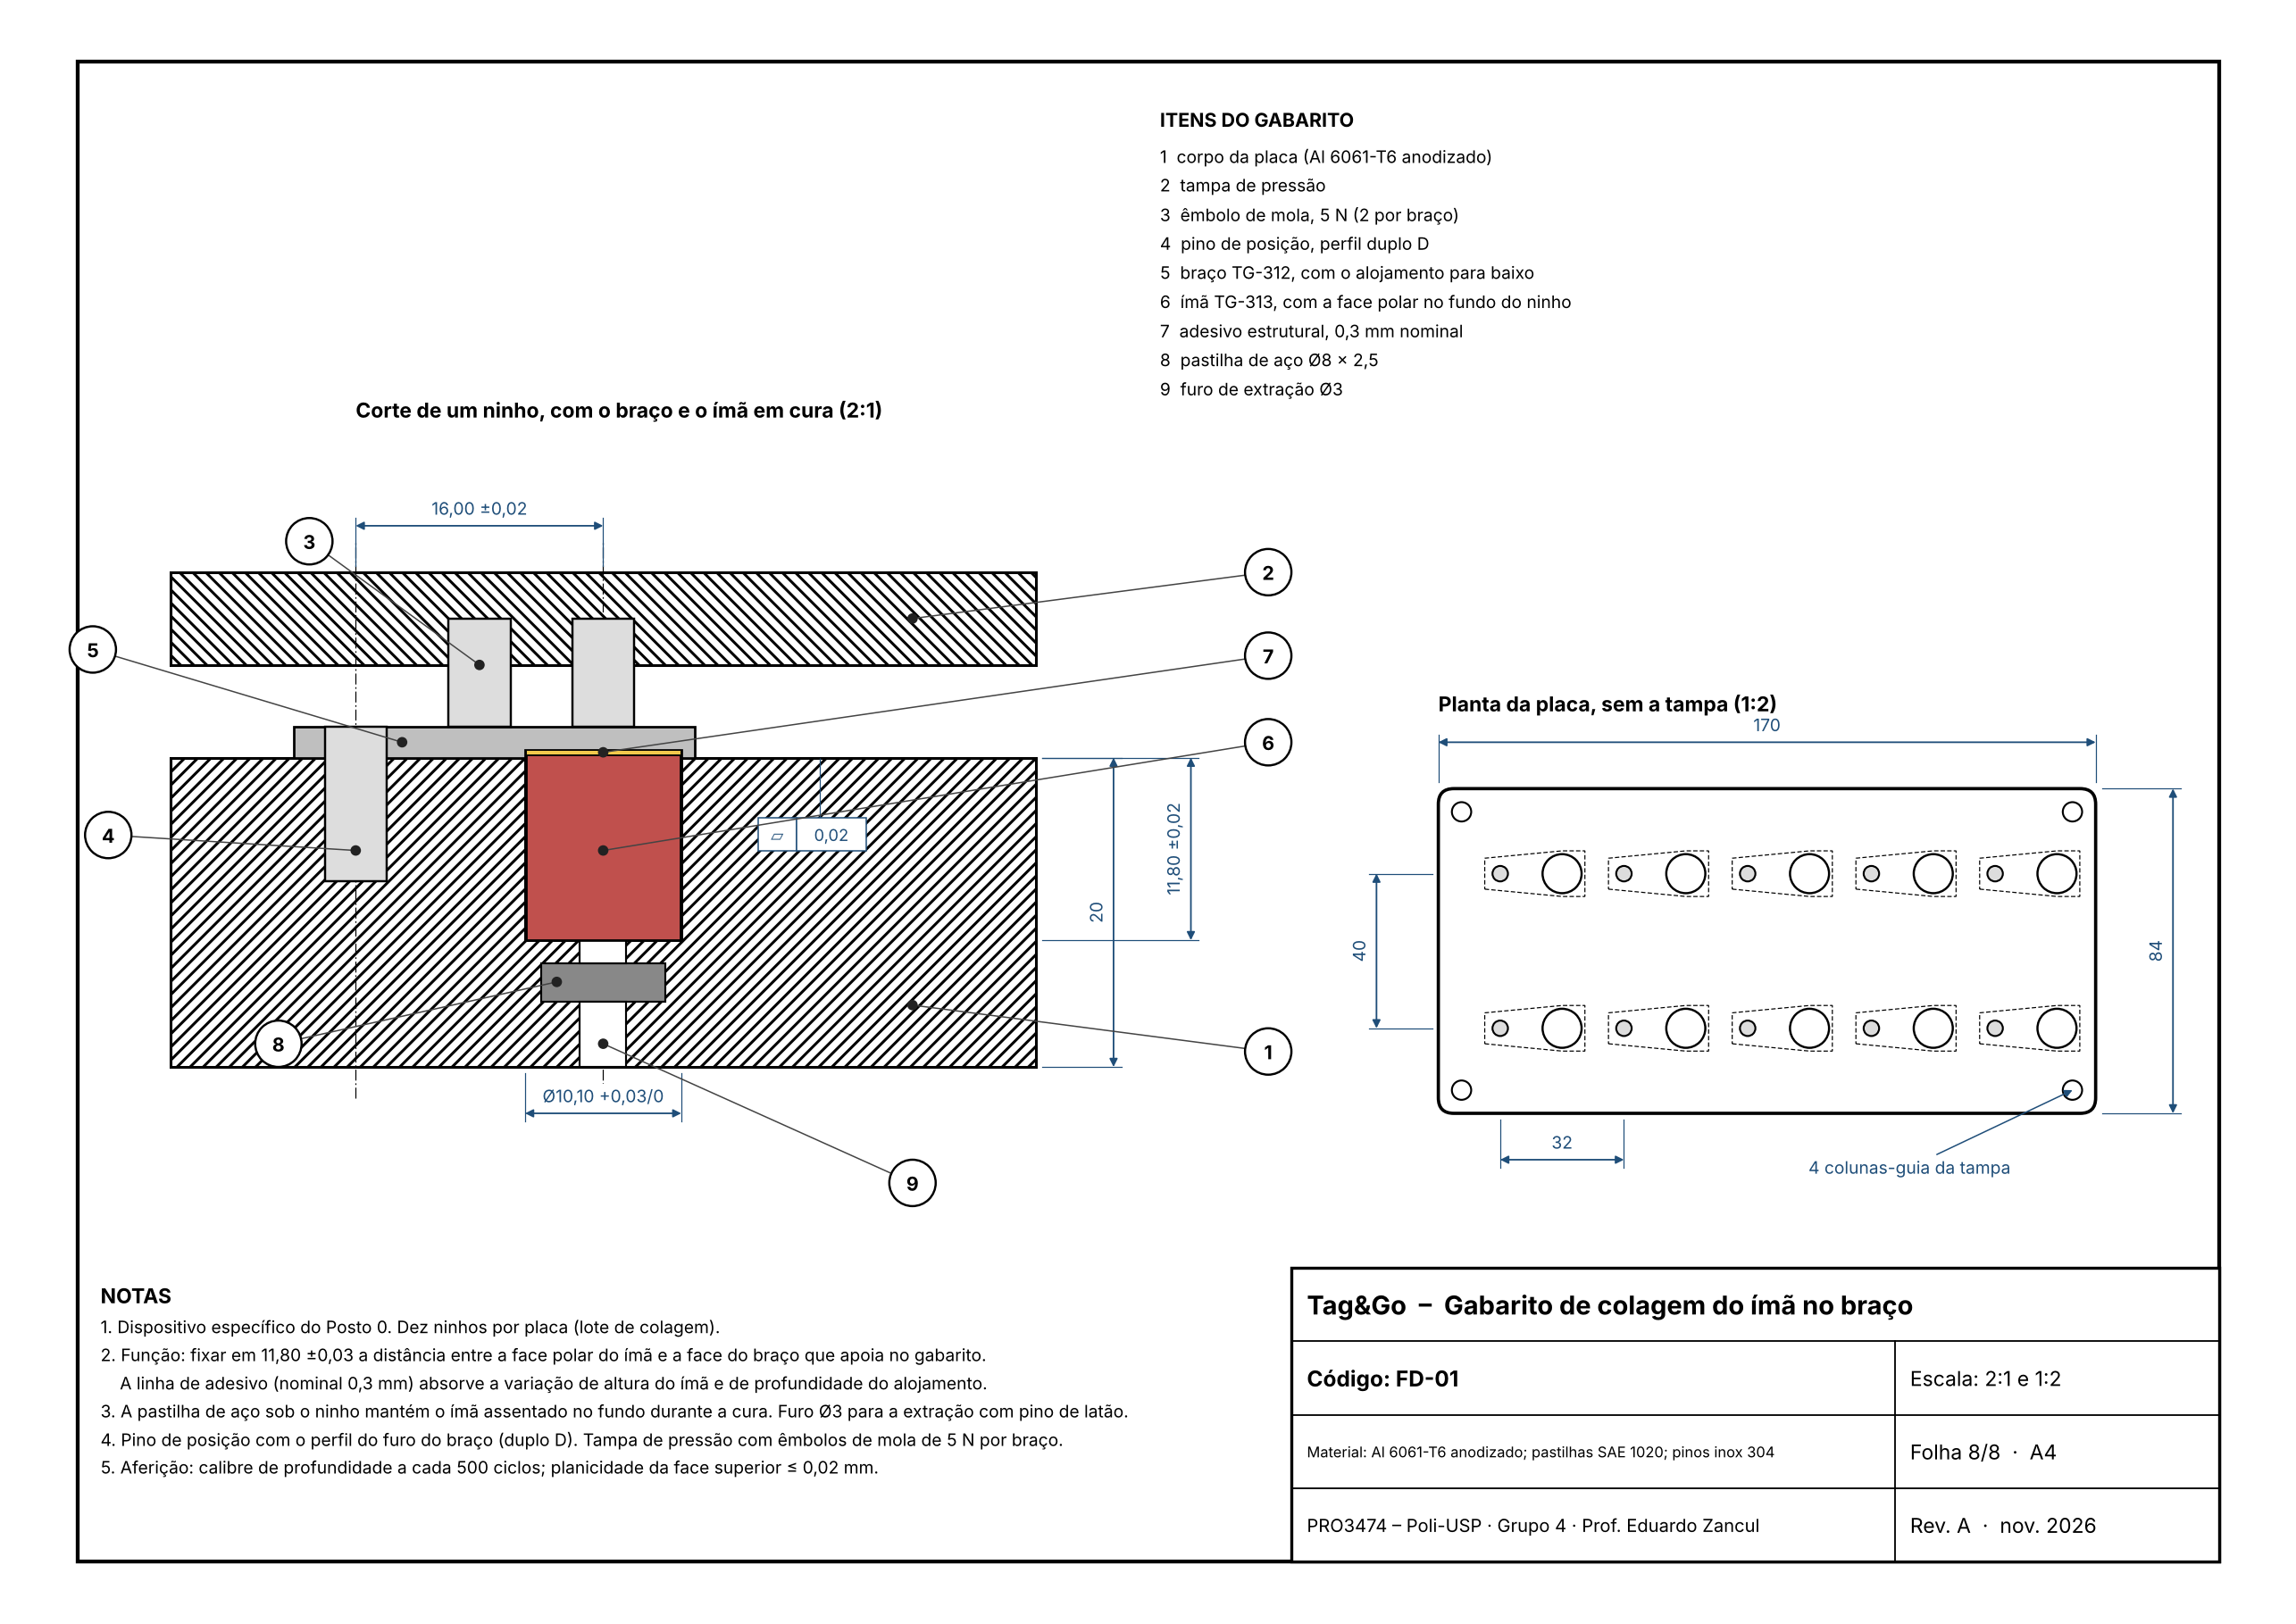
\includegraphics[height=0.86\textheight]{imagens/desenhos_execucao/fd01_gabarito.png}
    \source{Elaborado pelos autores (2026). Desenho gerado com apoio de ferramenta de IA.}
\end{figure}
\end{landscape}

Faltava resolver como manter o ímã no fundo durante a cura sem um grampo, que impediria a entrada do braço. A saída foi embutir uma pastilha de aço de baixo carbono sob cada ninho: ela atrai o ímã através de 1,5~mm de alumínio, força suficiente para assentá-lo e pequena o bastante para soltá-lo depois. Um pino com o perfil duplo~D do furo do braço posiciona o braço a 16,00~mm do eixo do ninho e impede que ele gire. A tampa de pressão desce por quatro colunas, e dois êmbolos de mola de 5~N por braço o mantêm apoiado na placa. Depois da cura, a placa é virada sobre uma base com dez pinos de latão, que passam pelos furos de $\varnothing$~3~mm do fundo e empurram os dez conjuntos de uma vez.

O corpo e a tampa são de alumínio 6061-T6 anodizado, que não interfere no ímã e solta bem o adesivo curado. O ninho tem 10,10~mm de diâmetro, com tolerância de $+$0,03~mm, para guiar o ímã de 10~mm sem prendê-lo.

\subsection{Uso e quantidade}
\label{subsec:disp_uso}

A Tabela~\ref{tab:disp_uso} detalha as operações 0.4 a 0.6 do plano macro.

\begin{table}[htbp]
    \centering
    \caption{Sequência de uso do gabarito FD-01}
    \label{tab:disp_uso}
    \footnotesize
    \renewcommand{\arraystretch}{1.3}
    \begin{tabularx}{\textwidth}{@{}
        c
        >{\RaggedRight\arraybackslash}X
        >{\RaggedRight\arraybackslash}p{4.6cm}@{}}
        \toprule
        \textbf{Passo} & \textbf{Ação} & \textbf{Ferramenta} \\
        \midrule
        1 & Limpar os ninhos & Haste de latão \\
        2 & Colocar um ímã em cada ninho e retirar o separador & Pinça não magnética \\
        3 & Aplicar o epóxi no alojamento de cada braço desengraxado & Dosador volumétrico \\
        4 & Encaixar os braços nos pinos, alojamento para baixo, e travar a tampa & Manual \\
        5 & Curar em estufa por 30~min a 60~$^\circ$C & Estufa de bandejas \\
        6 & Virar a placa sobre os pinos de extração e retirar os braços & Base de extração \\
        7 & Medir a altura de um braço por placa: 13,80~$\pm$0,03~mm & Relógio comparador em desempeno \\
        \bottomrule
    \end{tabularx}
    \source{Elaborado pelos autores (2026).}
\end{table}

Cada gabarito leva cerca de 40~min por ciclo, contando carga, cura e extração, e produz 15 braços por hora. Para 20 mil braços por mês em 280~h úteis, o posto precisa de 72 por hora, ou cinco gabaritos em giro. A equipe previu seis, para que um fique sempre em aferição: a profundidade dos dez ninhos é conferida com calibre de profundidade a cada 500 ciclos, e a planicidade da face, em desempeno, com limite de 0,02~mm.
